\documentclass[border=12pt]{standalone}
\usepackage{amssymb,amsmath}
\usepackage{tikz}
\usetikzlibrary{arrows.meta,positioning,shapes.multipart,shapes.geometric,calc,fit}

% Monochrome causal-graph house style of Renson, Dukes & Shahn (2026) and
% Knaus & Pfleiderer (2026): observed = solid outline, unobserved = dashed;
% solid directed edge = structural effect; dashed directed edge = "toggled"
% (assumed-absent) dynamic; treatment split into a SWIG node; the conditional
% parallel-trends statement made explicit with a difference node Delta Y(0).
\begin{document}
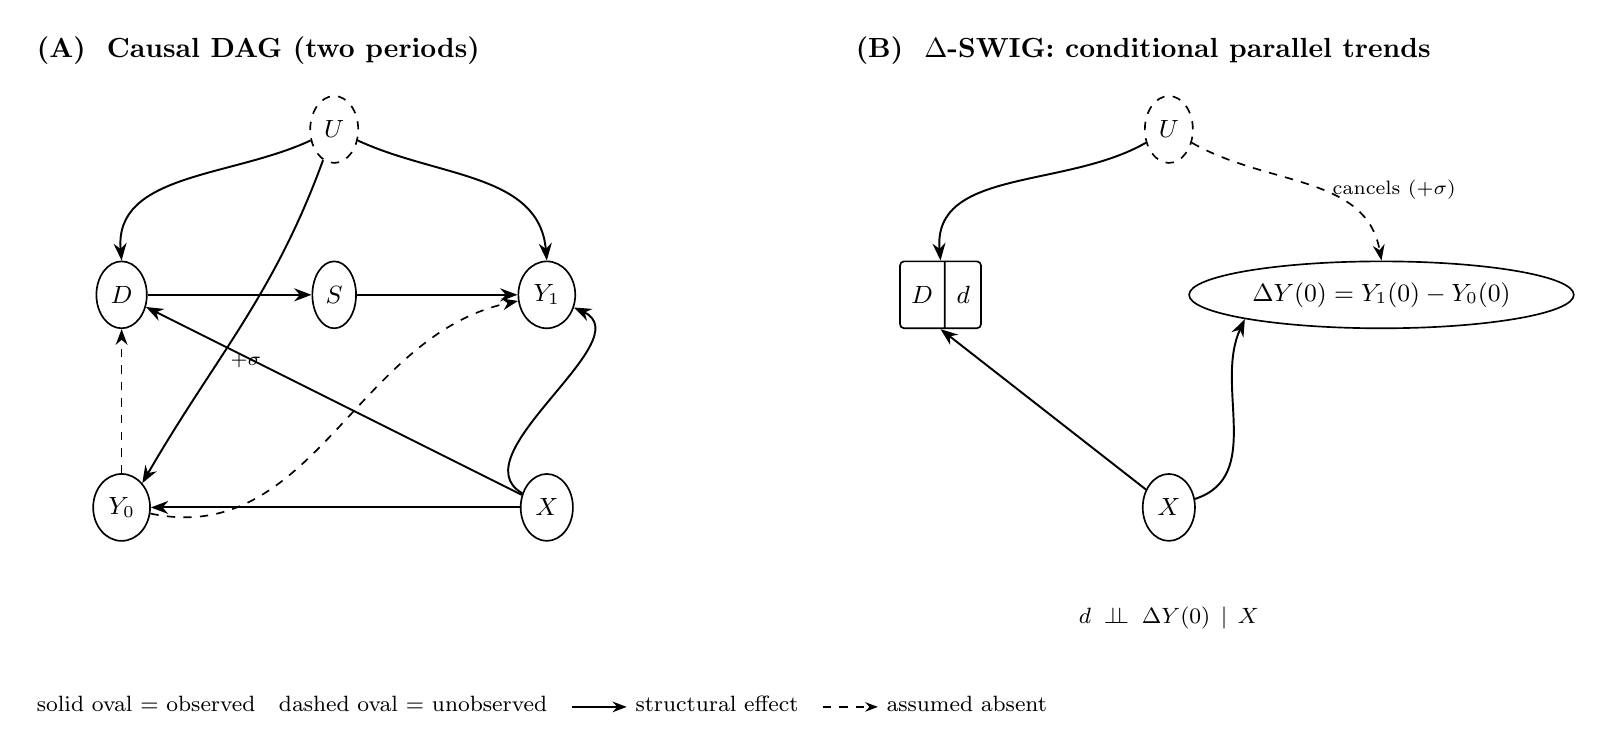
\begin{tikzpicture}[
  font=\small,
  >={Stealth[length=2.2mm]},
  obs/.style ={draw, ellipse, inner sep=2.5pt, align=center, line width=0.6pt, minimum height=8.5mm},
  lat/.style ={draw, ellipse, dashed, inner sep=2.5pt, align=center, line width=0.6pt, minimum height=8.5mm},
  swig/.style={draw, rounded corners=1.5pt, rectangle split, rectangle split parts=2,
               rectangle split horizontal, inner sep=4pt, line width=0.6pt, minimum height=8.5mm},
  eff/.style ={-{Stealth[length=2.2mm]}, line width=0.7pt},
  tog/.style ={-{Stealth[length=2mm]}, dashed, line width=0.6pt},
]

% ======================= Panel A : Causal DAG (two periods) =======================
\begin{scope}
  \node[lat] (U)  at (2.7, 3.2)  {$U$};
  \node[obs] (A)  at (0, 1.1)    {$D$};
  \node[obs] (M)  at (2.7, 1.1)  {$S$};
  \node[obs] (Y1) at (5.4, 1.1)  {$Y_1$};
  \node[obs] (Y0) at (0, -1.6)   {$Y_0$};
  \node[obs] (X)  at (5.4, -1.6) {$X$};

  % structural effects (solid)
  \draw[eff] (A) -- (M);
  \draw[eff] (M) -- (Y1);
  \draw[eff] (U) to[out=205,in=95] (A.north);
  \draw[eff] (U) to[out=250,in=60] node[pos=0.62,right=0.5pt,font=\scriptsize]{$+\sigma$} (Y0.north east);
  \draw[eff] (U) to[out=-25,in=95] (Y1.north);
  \draw[eff] (X) -- (A);
  \draw[eff] (X) to[out=150,in=-25] (Y1);
  \draw[eff] (X) -- (Y0);
  % assumed-absent (toggled) dynamics: state dependence and outcome->treatment feedback
  \draw[tog] (Y0) -- (A);
  \draw[tog] (Y0) to[out=-12,in=192] (Y1);

  \node[anchor=west, font=\bfseries] at (-1.2, 4.2) {(A)\ \ Causal DAG (two periods)};
\end{scope}

% ======================= Panel B : Delta-SWIG (conditional PT) =======================
\begin{scope}[xshift=10.4cm]
  \node[lat]  (U2) at (2.9, 3.2)  {$U$};
  \node[swig] (Aa) at (0, 1.1)    {$D$ \nodepart{two} $d$};
  \node[obs, minimum width=30mm] (DY) at (5.6, 1.1) {$\Delta Y(0)=Y_1(0)-Y_0(0)$};
  \node[obs]  (X2) at (2.9, -1.6) {$X$};

  \draw[eff] (U2) to[out=210,in=95] (Aa.north);
  % U enters both untreated potential outcomes additively (+sigma) and CANCELS in the difference:
  \draw[tog] (U2) to[out=-30,in=100] node[pos=0.55,right=1pt,font=\scriptsize]{cancels ($+\sigma$)} (DY.north);
  \draw[eff] (X2) -- (Aa.south);
  \draw[eff] (X2) to[out=18,in=-115] (DY.south west);

  \node[anchor=west, font=\bfseries] at (-1.2, 4.2) {(B)\ \ $\Delta$-SWIG: conditional parallel trends};
  \node[align=center, font=\footnotesize] at (2.9, -3.0)
       {$d \;\perp\!\!\!\perp\; \Delta Y(0)\,\mid\, X$};
\end{scope}

% ======================= shared key =======================
\node[anchor=west, font=\footnotesize] at (-1.2, -4.1)
   {solid oval = observed\quad dashed oval = unobserved\quad
    {\tikz[baseline=-0.5ex]\draw[-{Stealth[length=1.8mm]},line width=0.7pt](0,0)--(0.7,0);} structural effect\quad
    {\tikz[baseline=-0.5ex]\draw[-{Stealth[length=1.6mm]},dashed,line width=0.6pt](0,0)--(0.7,0);} assumed absent};
\end{tikzpicture}
\end{document}
